\documentclass[12pt]{article}
 
\usepackage[margin=1in]{geometry} 
\usepackage{amsmath,amsthm,amssymb}
\usepackage[normalem]{ulem}
\usepackage[table,xcdraw]{xcolor}
\usepackage{tablefootnote}
\usepackage{lscape}
\usepackage{wrapfig}
\usepackage{caption}
\usepackage{graphicx}
\usepackage{setspace}
\usepackage{titling} 
\usepackage{lmodern} 
\usepackage[backend=biber, style=authoryear, maxcitenames=2, uniquename=false]{biblatex}
\addbibresource{references.bib}
\usepackage[utf8]{inputenc}
\usepackage{url}
\usepackage[hidelinks]{hyperref}
\usepackage{bbm}
\usepackage{adjustbox}
\usepackage{booktabs}
\usepackage{tocloft}

 
\newcommand{\N}{\mathbb{N}}
\newcommand{\Z}{\mathbb{Z}}
\onehalfspacing
\setlength{\parindent}{0pt}
\setlength{\parskip}{1em}
\setlength{\cftbeforesecskip}{2pt}
\setlength{\cftbeforesubsecskip}{1pt}


 
% --------------------------------------------------------------
%                         Start here
% --------------------------------------------------------------

\title{
\centering
\textbf{\LARGE Farewell to the American Dream --}\\
\textbf{\LARGE How Endogenous Feedback Loops Shape Wealth Accumulation}
}

\pretitle{
\begin{center}
\noindent\rule{\textwidth}{0.4pt}
\vspace{0.1em}
\end{center}
}
\posttitle{
\begin{center}
\vspace{0.5em}
\noindent\rule{\textwidth}{0.4pt}
\par\vspace{1.5em}
{\Huge\textbf{Master Thesis}} \\
\vspace{1.5em}
{\Large\textbf{Paris School of Economics}} \\
\vspace{1em}
{\Large\textbf{Analysis and Policy in Economics}}
\end{center}
}

\author{{\large Łukasz Krzempek}} 
\date{June 2025}

\begin{document}

\maketitle

\vfill

\begin{center}
\begin{tabular}{ll}
Supervisor: & Prof. Edouard Challe \\
Referees:   & Prof. Julien Matheron \\
            & Prof. Pau Roldan \\
\end{tabular}\\[0.5em]
\end{center}

\newpage

\begin{abstract}
\noindent
This thesis investigates the endogenous origins of wealth inequality through the lens of a partial equilibrium heterogeneous agents model with non-homothetic utility, Epstein-Zin preferences, and portfolio choice. Departing from traditional explanations based on ex-ante heterogeneity, the model emphasizes a dynamic mechanism in which wealthier individuals both save more and earn higher returns due to lower relative risk aversion. By incorporating non-homothetic bequest motives and allowing for investment in risky assets, the model successfully replicates the empirical wealth distribution in the United States, including its heavy right tail and the observed wealth-return gradient. The framework also offers novel insights into social mobility. Simulations reveal extreme persistence at the top: agents starting in the top 0.1\% almost never exit, while upward mobility into this group remains virtually nonexistent over multiple generations. To assess the relevance of the key mechanisms, the benchmark model is systematically compared to alternative specifications: excluding either non-homothetic preferences or endogenous portfolio choice. These counterfactuals demonstrate that both components are crucial for reproducing empirical wealth concentration.

\vspace{1em}
\noindent\textbf{Keywords:} Wealth inequalities; Portfolio choice; Investment risk; Household finance; Non-homothetic preferences; Aiyagari models; Heterogenous agents models

\vspace{0.3em}
\noindent\textbf{JEL Codes:} D31; D11; D81; E21; D91; G11
\end{abstract}

\newpage
\tableofcontents
\newpage
% --------------------------------------------------------------
%                         Content
% --------------------------------------------------------------
\section{Introduction}
\label{sec:introduction}

Wealth inequality in contemporary developed economies appears to have reached its highest levels since the advent of modern capitalism.\footnote{The end of World War II is often treated as a conventional point of reference.} Regardless of whether inequality is measured using the traditional Gini coefficient or the increasingly popular metric of top wealth shares, current levels are historically unprecedented and reflect a pronounced upward trend beginning in the 1970s and 1980s (see, e.g., \textcite{piketty2014}, \textcite{piketty2020}, \textcite{saez2016}, \textcite{lakner2013}). In the United States, the wealth share of the top 1\% rose from approximately 25\% in 1980 to nearly 40\% by 2010. The increase is even more striking for the top 0.1\%, whose share grew from under 10\% in the 1970s and 1980s to well above 20\% today. This trend is particularly concerning given its apparent persistence. Excessive wealth concentration is widely regarded as undesirable — not only from the standpoint of various ethical theories of social justice, but also due to its implications for the stability of institutions underpinning Western liberal democracies. Importantly, wealth inequality is not merely an economic issue: the accumulation of wealth, especially in the upper tail of the distribution, tends to translate into non-market forms of power (e.g., political influence), shaping institutional rules and constraints that are typically abstracted away in economic models through assumptions such as perfect competition or the absence of informational frictions.

Traditionally, wealth inequality has been attributed to heterogeneity in both labor and capital income. While disparities in labor income fall within the well-established domain of labor economics—and largely account for social mobility within the lower and middle segments of the distribution—capital income plays a central role in shaping the evolution of top fortunes and the Pareto tail of the wealth distribution. As such, it is arguably the key driver of the most dynamic and persistent forms of inequality. It is important to note that, within the mainstream framework, the distribution of wealth is not fundamentally shaped by saving behavior. Under standard homothetic preferences, as demonstrated by \textcite{gorman1953}, income expansion paths are linear, and marginal propensities to consume (MPCs) remain constant across income levels. Although standard incomplete markets (SIM) models with borrowing constraints can generate declining MPCs near the constraint, saving behavior quickly converges to linearity away from it. This implies that differences in saving behavior alone cannot account for the stark divergence in wealth accumulation between the middle class and the wealthiest households.

This study departs  from the aforementioned standard in two key ways. First, I introduce non-homothetic preferences as proposed by \textcite{straub2019} to induce MPCs decreasing with wealth. As a result, wealthier agents save a larger fraction of their income, introducing an additional mechanism that amplifies wealth inequality. Second, I exploit the decreasing risk aversion property of Straub preferences by introducing portfolio choice between safe and risky assets. I follow \textcite{epstein1989} in defining recursive utility that disentangles the intertemporal elasticity of substitution and the risk aversion in order to match the equity premium. Together, these two mechanisms produce a rising risky asset share with wealth, consistent with empirical evidence. For instance, \textcite{scf2022} reports that 92\% of directly held stocks in the United States are owned by the top 10\% of households. Due to the equity premium, this concentration of risky assets translates into a positive correlation between wealth and average return—a phenomenon receiving increasing attention in the literature, as highlighted by \textcite{fagereng2020}. In their comprehensive structural decomposition of U.S. wealth inequality dynamics, \textcite{hubmer2021} impose this return-wealth gradient exogenously. In contrast, the presented model aims to generate it endogenously.

My model closely replicates the empirical distribution of wealth, particularly capturing the extreme concentration at the top and the heavy-tailed nature of observed data. In the stationary equilibrium, the shares of wealth held by the top 1\% and top 0.1\% of households align remarkably well with estimates from the World Inequality Database. Crucially, the model achieves this level of realism without relying on ex-ante heterogeneity in preferences, productivity, or investment access - mechanisms that are commonly referenced to generate skewed wealth distributions in the literature.

To demonstrate the central role of Straub-type preferences and endogenous portfolio choice, I compare the full model against two simplified variants: one excluding utility from bequests, and another omitting risky asset allocation. This comparison highlights that both declining marginal propensities to consume and scale-dependent returns are essential ingredients for explaining wealth inequality.

In addition to matching the wealth distribution, the model successfully reproduces a key empirical regularity: the increasing share of risky assets held by wealthier households, which translates into a positive relationship between wealth and realized returns. This mechanism, driven by declining relative risk aversion, provides a parsimonious explanation for the rising dominance of the very wealthy in recent decades. By endogenizing the link between wealth and return, the model helps to bridge the gap between the macroeconomic literature on inequality and the micro-foundations of investment behavior. Furthermore, the model offers insight into the dynamics of social mobility: it captures the extreme persistence of wealth at the very top of the distribution and the limited upward mobility for the majority of households. 

These findings offer a natural entry point into normative considerations, suggesting that the long-run risks of unmitigated capital concentration may outweigh the short-run efficiency costs typically associated with capital income and monopoly profit taxation. This perspective resonates with recent contributions in optimal taxation theory (summarized by \textcite{bastani2020}), which emphasize the role of capital returns in driving inequality and argue for progressive taxation not merely on distributional grounds, but as a corrective to endogenous structural divergence. 

The paper is organized as follows: Section~\ref{sec:literature} provides a literature review on dynamics of wealth inequalities, risk aversion and investment behavior, and relationships between wealth and return. Section~\ref{sec:model} outlines the model setup and demonstrates fundamental properties of employed preferences. Section~\ref{sec:calibration} presents the calibrated values of parameters, and Section~\ref{sec:analysis} performs a full quantitative analysis of the model and compares it with models without decreasing MPCs and decreasing risk aversion. Section~\ref{sec:conclusion} concludes.

\section{Literature}
\label{sec:literature}

\subsection{Dynamics of wealth distribution}

Throughout the last 35 years there have emerged many attempts to theoretically capture the roots of empirical facts observed around the evolution of wealth. \textcite{piketty2015} focus on the wealth-to-income ratio, showing that at the turn of the 20th century, it no longer follows either classical Kaldor stylized fact \parencite{kaldor1957}, claiming it to be constant, or the famous Kuznets curve \parencite{kuznets1955}, which would imply it to decrease in developed countries. Instead, the ratio, reaching after World War II in developed countries values around 2-3, today often exceeds 5-6. They use an overlapping-generations model with simplified linear laws of motion of wealth distribution and inheritance to demonstrate the possible future trajectory of wealth concentration processes observed in past data. A commensurate approach is applied by \textcite{gabaix2016}, who discuss the random growth mechanism\footnote{Basing on Gibrat's law \parencite{gibrat1931}, postulating independence of size and growth rate of a given phenomenon. The most frequent examples addressed with the law are firms' sizes and cities' populations in the US.}, widely present in the literature as the generator of Pareto-tailed distributions, and modify it to speed up transitional dynamics so that it matches the data. They add two effects: type dependence, stipulating differentiation in distributions of random growth rates among individuals, and scale dependence, advocating for dependence of the distribution of the current wealth. As the next subsections will discuss, identification and distinguishing of these effects are one of the substantial challenges for both empirical and theoretical analysis of wealth distribution evolution.

These models are, however, based on ex-ante assumed decision rules and abstracting from market interactions, and hence do not fit into the mainstream rational expectations dynamic general equilibrium framework. The standard structural micro-founded tool used to investigate inequalities (and household heterogeneity in general) is the Standard Incomplete Markets (SIM) or Bewley-Hugget-Ayiagari model \parencite{bewley1977, huggett1993, aiyagari1994} with ex-ante identical agents, differing in idiosyncratic endowment/productivity following a Markov process. These types of models features, however too high social mobility compared to the data, and, most importantly, the wealth distribution produced by the model does not correspond to the empirical observations, with the most important element absent being a Pareto tail of exceptionally wealthy individuals. Numerous extensions were able to fabricate distributions closer to reality, with arguably the most prominent being \textcite{krusell1998}, who managed to introduce the aggregate shocks into the Aiyagari economy. \textcite{castaneda2003} focus on the role of labor income inequalities, adding "top income state" to the standard discretized Markov process. High persistence of such a state enhances the long tail of wealth distribution and limits social mobility. \textcite{kaymak2016} also consider the effects of income inequality, in particular highlighting the role of the tax system (primarily declining capital taxation) in the recent rise of wealth inequalities.

The comprehensive decomposition of discussed trends is provided by \textcite{hubmer2021}, who use the transition path in an Ayagiari-like model to decompose the aggregate effect into particular factors and attribute them to the percentage share in reaching from the 1960s wealth distribution to the current macroeconomic situation. They find out that the major driver of the inequality emergence is the policy change involving taxation - most importantly decreasing marginal tax rates and general tax progressivity. However, apart from the policy analysis, the structural economic effects of two essential income sources - labor and capital - appear interesting. First, according to their decomposition, earnings inequality tends to increase wealth inequality,\footnote{Earnings inequality is modeled, similar to \textcite{castaneda2003}.}  but mostly in terms of decreasing the wealth share of the bottom 50\% and increasing that of the top 10\%, as labor earnings are only weakly correlated with wealth. Interestingly, earnings risk itself has an inequality-reducing effect, as it incentivizes even poorer households to keep precautionary savings. On the side of the capital income, the model includes a positive correlation between wealth and return (discussed broadly in the next section), which is another strong inequality-increasing factor.

\subsection{Wealth and return on assets}

As the capital income channel is considered to play an essential role in determining top wealth shares, the proper identification of the link between wealth and return on that wealth is of particular importance. It is not surprising that empirical research indicates the positivity of that relationship. If wealthier individuals had automatic access to higher return rates, the emerging inequalities would become increasingly difficult to contain. It is, however, not sufficient to infer whether there is such an inherent divergence engine in the investment mechanism: the reverse causal relationship, based on type dependence, appears no less likely. \textcite{fagereng2020} find for Norwegian administrative data that the 90th percentile of wealth features net-of-tax returns higher by 10 percentage points than the 10th percentile. They attribute a significant part of heterogeneity in returns to natural differences in information, entrepreneurship, and financial sophistication, hence advocating that differentiated return rates are a transmission mechanism from ex-ante disparity into wealth distribution.

A similar mechanism is demonstrated in more detail by \textcite{benhabib2019}, who provide a partial equilibrium model with a stochastic return rate (agent-specific and constant through lifetime), being one of the factors inducing skewed wealth distribution. They then consider also the direct influence of wealth on return, endowing the initially drawn capital income rate with a wealth percentile-dependent component. The latter improves the model's fit to the data. That, however, fails to improve the matching of social mobility, as the saving decisions of modeled agents compensate for higher/lower rates of return. Another empirically confirmed result in the paper is the strong intergenerational correlation of idiosyncratic return rate, negatively impacting intergenerational social mobility.

Comparable evidence, but for Swedish data, is provided by \textcite{calvet2007} and \textcite{bach2020}. The first paper shows that more efficient investment strategies of wealthier households are connected with higher risk taken. That is however not attributed to the different levels of risk aversion across households, but rather exogenous characteristics similar to those mentioned by Fagereng et al. - authors argue that the distribution of stochastic risky returns is not the same for households with different levels of financial sophistication: for example, less educated agents may expect a lower return from the stock market, hence their participation in these instruments is low. The second paper makes several original contributions to the wealth return dependence puzzle, i.a. undermines the influence of exceptional “investment skills” of individuals and attempts to reconcile the type and scale dependence in returns by comparing twin siblings, and showing that even among them the expected correlation between wealth and return is not significantly lower.

The topic of risk aversion is tackled by \textcite{kekre2022}, who introduce heterogeneous relative risk aversion coefficients in the HANK model, finding that with two available savings instruments, nominal bonds and capital, households with a high wealth to labor income ratio are those that were endowed with lower RRA.

Concluding, we can distinguish two essential explanations of the correlation between wealth and equity present in the literature:

\begin{enumerate}
    \item Type dependence - some households are wealthier than others because they have access to higher returns on their savings. The reason for the latter is either some exogenous factor (financial sophistication, entrepreneurship) or pure luck
    \item Scale dependence - return rate is an increasing function of wealth, either because some investment instruments are available only for rich enough households, or because agents face decreasing risk aversion, making the optimal portfolio of wealthy households riskier and therefore yielding a higher average return.
\end{enumerate}

Of course, the most plausible explanation is the interplay of both-sided causal effects. For example, financial sophistication can be endogenized by including investment in financial literacy, like in the stylized model of \textcite{spataro2017}. The major challenge is then to decompose the spiral and obtain the relative strength of each effect. Studies like \textcite{gaillard2023}, including both effects and showing the opposite forces they exert on the e.g. optimal capital tax rate, seem to become a particularly prosperous field.

\subsection{Savings and investment decisions}

Saving behavior used to be less considered in the context of wealth distribution, as under homothetic preferences, marginal propensities to save do not differ across the population. The only agents with different MPSs are those close to the borrowing constraints, who affect the distribution and aggregate variables the least, as they hold the lowest assets (as noticed in the approximate aggregation result of \textcite{krusell1998}). Therefore, most attempts to incorporate the role of heterogeneity in savings rates relied on ex-ante differentiation of discount factors \textcite{benhabib2011, carroll2017}, calibrating it to match wealth distributions and the distribution of MPCs. However, as discount factors are not directly measurable, it is hard to assess the extent to which such an explanation is plausible.

Despite the popularity of the Permanent Income Hypothesis, dating back to \textcite{friedman1957}, it is hard to claim that consumption smoothing and precaution are the only motives of accumulating wealth, especially for the very richest. The empirical observations do not support the claim that MPCs are constant. \textcite{dynan2004} pioneered in showing that saving rates differ significantly in wealth. \textcite{straub2019} improved their empirical strategy using a higher-quality PSID dataset to show that consumption is, in fact, concave in permanent income, with an elasticity of 0.7. Straub is also the first who step against the homotheticity in the formulation of the notion of preferences. In his model, agents derive utility not only from consumption, but also from bequests they leave to their offspring when they die. Such an economy features important deviations from classic models: most importantly, as inequality increases, the wealth / GDP ratio increases as well, and the equilibrium interest rate declines.

An additional and increasingly central channel through which wealth inequality can evolve is the heterogeneity in investment behavior- particularly, in the allocation of wealth between safe and risky assets. While savings behavior alone may not suffice to generate the heavy-tailed wealth distributions observed empirically, the interaction between saving motives and portfolio choice plays a crucial role. In classical models of portfolio selection under uncertainty, such as those developed by \textcite{samuelson1969} and \textcite{merton1969}, agents with constant relative risk aversion (CRRA) optimally allocate a fixed proportion of their wealth to risky assets, regardless of their income or wealth level. This result, sometimes referred to as the mutual fund theorem, implies that portfolio composition should be homogeneous across households with similar preferences.

However, empirical evidence strongly contradicts this prediction. Studies consistently find that participation in risky asset markets increases with wealth, and that richer households not only hold more risky assets in absolute terms, but also allocate a larger share of their portfolios to them \parencite{campbell2002,fagereng2020}. This discrepancy has prompted several attempts to reconcile theory with observed portfolio heterogeneity, e.g. through life-cycle, behavioral, and market participation frictions. \textcite{cocco2005} show that once labor income is made stochastic and not fully insurable, younger and poorer agents optimally choose lower risky shares - even under CRRA preferences - due to the implicit correlation between labor income and equity returns. Similarly, \textcite{constantinides1986} demonstrates that habit formation preferences can account for limited participation and lower risk-taking among less wealthy households. In his model, current utility depends not only on current consumption but also on a “habit stock,” typically linked to past consumption levels, which generates an endogenous precautionary motive. \textcite{heaton2000} emphasize the role of undiversifiable idiosyncratic risk, particularly entrepreneurial or labor income risk, in generating persistent heterogeneity in portfolio composition. Using calibrated models with incomplete markets, they show that such risks discourage equity investment even among agents who are otherwise unconstrained. \textcite{vissing2002} investigates why many households abstain from holding risky assets despite favorable average returns and proposes that participation costs, such as information or transaction frictions, can account for the limited asset market participation.

To advocate for the theory claiming that equity ownership structure contributes crucially to scale effects of return from wealth, and through that to wealth inequalities per se, the evidence for the essential and increasing role of equity returns is required. Such evidence is provided by \textcite{barkai2020}, who demonstrates empirically that monopolistic (or pure) profits share increased from 1984 to 2014 by 14.600 USD per employee, offsetting both labor share (declining by 11\% in the given period) and capital share (22\% decline). \textcite{eggertsson2021} provide estimates of 5-year moving averages of factor shares according to which pure profit share increased from 3\% around 1985 to 17\% in 2015, so almost six times. They point it out as one of the major long-run trends of the contemporary economy and attribute it to effects such as a decline in natural interest rate and an increase in wealth-to-income ratio.

Another evidence, provided by \textcite{deLoecker2020}, directly addresses the level of markups. According to firm-level data they investigated, aggregate markups rose from 21\% above marginal cost in 1980 to 61\% in 2016. They attribute the effect mostly to gaining significantly more market share by high-markup firms and fattening the upper tail of the markup distribution. What is even more crucial from the point of view of stock market returns, they also find a tremendous growth in average profit rate - from 1\% to 8\% in the corresponding period.

Incorporation of monopoly power into heterogenous agents setup, capable of investigating the inequalities, was performed also by \textcite{colciago2019} and \textcite{brun2017}, who respectively introduce oligopoly with an endogenous number of firms and explain rising Tobin's Q coefficient\footnote{Which is arguably the most important explanation of rising wealth to income ratio, famously observed by \textcite{piketty2014}.}. \textcite{piketty2014} expresses a similar view on monopoly power's influence on wealth to income ratio, showing the rising disparity between wealth and productive capital and attributing it to discounted monopoly (and other) rents.

\section{Model}
\label{sec:model}

This section first presents Straub preferences and general properties of intertemporal substitution and portfolio choice under this setup. Then I establish a more general model that nests Straub preferences inside Epstein-Zin recursive utility function, which will be calibrated and investigated in general equilibrium framework.

\subsection{Straub preferences in dynamic setting}
\label{subsec:simple_model}

\textbf{Setup.} Consider the standard dynamic stochastic infinite-horizon consumption-savings problem, but each period, agents face a constant probability of death $\gamma$. When dying, agents derive utility from bequests they leave to their offspring, equal to total wealth held in the period of death. Total expected utility, maximized by agents, is hence given by:

\[
\max_{\{c_t, W_t\}_{t=0}^{\infty}} \mathbb{E}_0 \sum_{t=0}^{\infty} \beta^t \left( (1-\gamma)u(c_t) +  \gamma \mathcal{U} \left( W_t \right)\right)
\]

Where $u$ is the utility from consumption, and $\mathcal{U}$ - from bequests. \textcite{straub2019} shows that under CRRA  forms of both functions:

\[
u(c) = \frac{c^{1 - \theta}}{1 - \theta}, \quad
\mathcal{U}(W) = A \frac{W^{1 - \eta}}{1 - \eta}
\]

bequests are effectively a luxury good if $\eta<\theta$.

Each period, agents face an autocorrelated idiosyncratic productivity shock $z_t^i$ as in \textcite{aiyagari1994}. The budget constraint is hence:

\[
w_t z_t^i + W_t^i = c_t^i + s_t^i
\]

where $w_t$ is wage in period $t$ and $s_t^i$ are savings of an individual $i$, such that $W_{t+1}^i = RET_{t+1}^i s_t^i$ with $RET_t^i$ being the individual (possibly) stochastic return on wealth in period $t$.

\textbf{Solution and consumption function.} The problem can be expressed with a Bellman equation:

\[
V\left(W_t^i, z_t^i\right) = (1 - \gamma) 
\max_{c_t^i \in [0,z_t^i w_t+W_t^i]} 
\left[ 
    u(c_t^i) 
    + \beta \mathbb{E}_t \left[
        V\left(W_{t+1}^i, z_{t+1}^i
        \right)
    \right]
\right]
+ \gamma \mathcal{U}(W_t^i)
\]

where $W_{t+1}^i = RET_{t+1}^i (w_t z_t^i + W_t^i - c_t^i)$. That allows us to derive the Euler Equation:

\[
u'(c_t^i) = \beta \mathbb{E}_t \left[ RET_{t+1}^{i} \left( (1 - \gamma) u'\left(c_{t+1}^{i}\right) + \gamma \mathcal{U}'\left(W_{t+1}^{i}\right) \right) \right]
\]

Suppose for now that $RET_{t+1}^i = R$, so the return is deterministic and constant. The right-hand side of the Euler Equation consists then of the standard future marginal utility $\beta R \mathbb{E}_t \left[ u'\left(c_{t+1}^{i}\right) \right]$ and the "wedge" $\beta R \gamma \mathbb{E}_t \left[ \mathcal{U}'\left(W_{t+1}^{i}\right) - u'\left(c_{t+1}^{i}\right) \right]$. The sign of this "wedge" depends on the sign of the difference $\mathcal{U}'\left(W_{t+1}^{i}\right) - u'\left(c_{t+1}^{i}\right)$, which represents two offsetting effects: direct utility from possible bequests, which incentivizes the agent to save more, and lost utility of future consumption in case of death, which urges them to consume more today, similarly to life-cycle consumption profile in OLG models (as in \textcite{yaari1965} modification of classic \textcite{modigliani1954} analysis). Numerical analysis shows that for $\eta<\theta$ and $A>0$, this results in a policy function for consumption that is concave in wealth (see \autoref{fig:cons_function} below).

\begin{figure}[h]
    \centering
    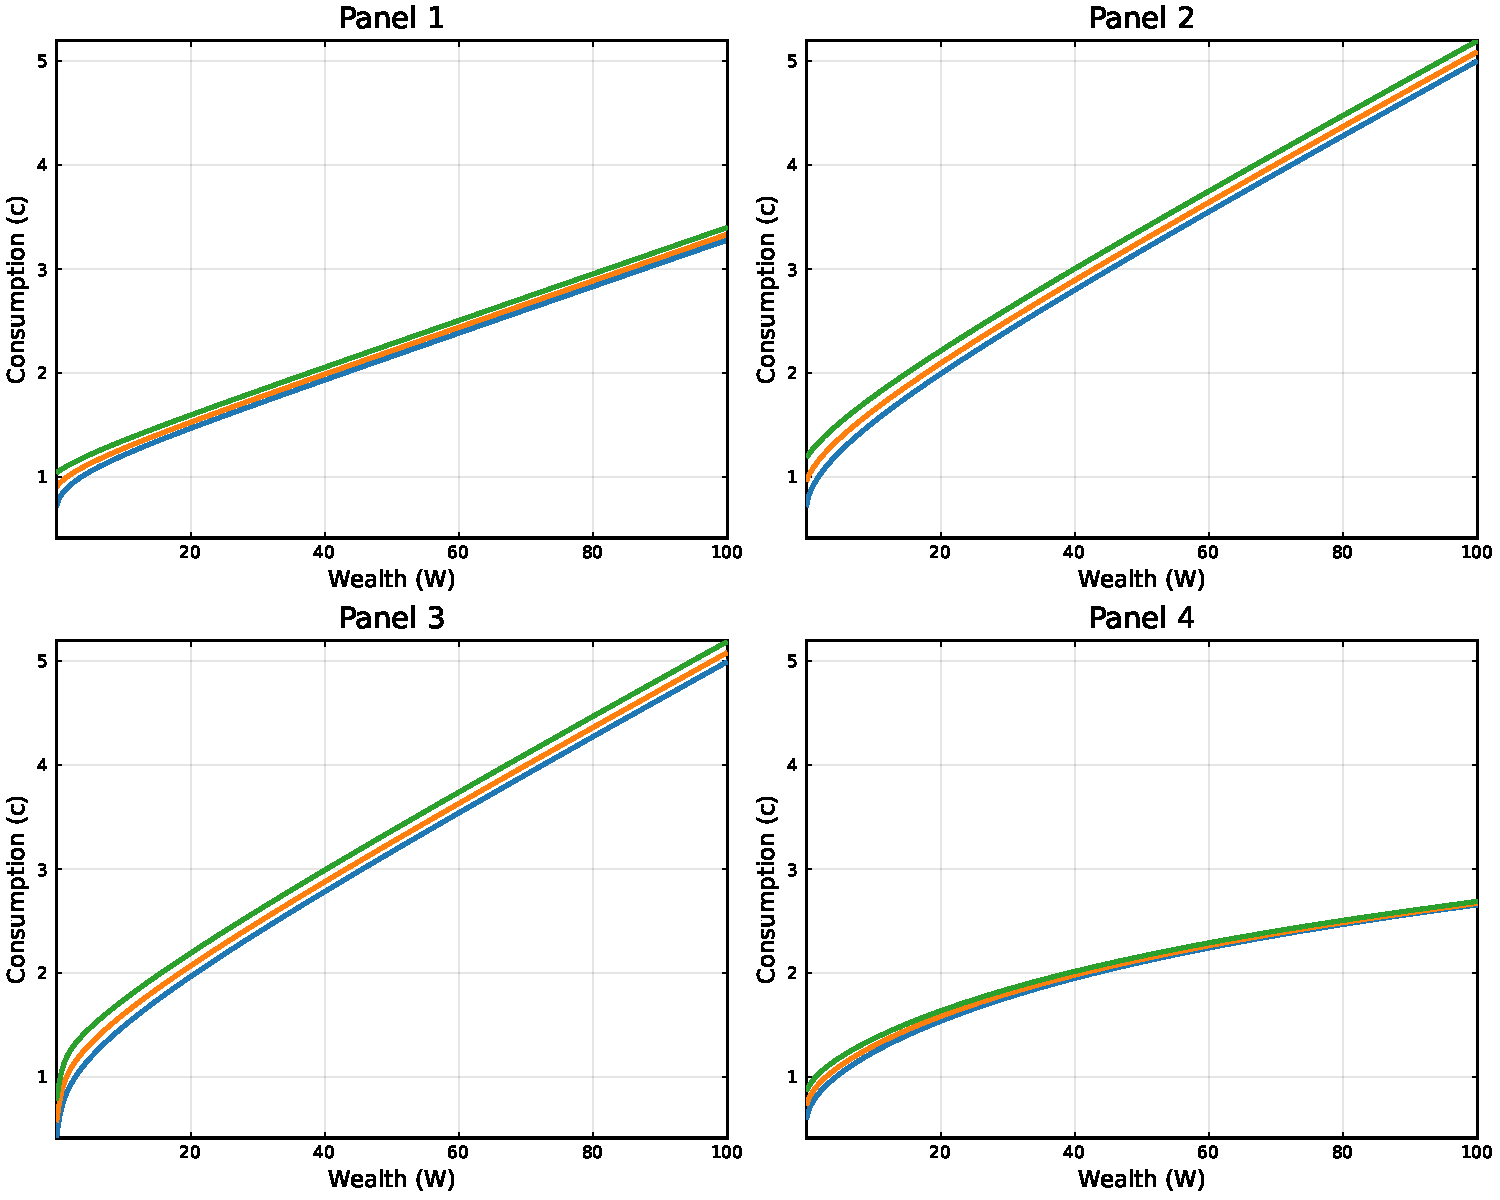
\includegraphics[width=1.0\textwidth]{figure_1.pdf}
    \caption{Consumption functions for homothetic and non-homothetic preferences}
    \label{fig:cons_function}
\end{figure}

Panel 1 shows the standard Aiyagari case without mortality. Panel 2 adds a constant probability of death, but without utility from bequests, so only the negative effect is present, effectively increasing the discount rate. Panel 3 adds utility from bequests, but keeping $\eta=\theta$. Saving behavior is then still asymptotically linear. Finally, in Panel 4, $\eta$ is lower than $\theta$, which leads to concavity in the consumption function.

\textbf{Risk aversion and portfolio choice.} Let's depart now from the assumption that the agent saves in a safe asset with a deterministic return only. Instead, they face an intratemporal portfolio choice between a safe asset (claims to capital) with return $R_t^i$ and a risky asset $S_t^i$ with expected gross return $1 + E_{d_t}$ and standard deviation $\sigma_{d_t}$. It can be interpreted as an investment in the stock market that pays idiosyncratic stochastic dividends $d_t^i$, assumed to be i.i.d. across individuals and independent between periods. We can hence denote with $\varphi$ portfolio share of the risky asset, meaning that $k_t^i=(1-\varphi) s_t^i$ and $S_t^i=\varphi s_t^i$. Next period wealth is then $W_{t+1}^i=R_{t+1}k_t^i + (1+d_{t+1}^i)S_t^i$ and the idiosyncratic return is $RET_{t+1}^i=(1-\varphi) R_{t+1} + \varphi(1+d_{t+1}^i)$. First Order Condition of the Bellman equation with respect to $\varphi$ gives then the intratemporal choice:


\[
\mathbb{E}_t \left[ 
\left( (1 - \gamma) \, u'\left(c_{t+1}^i\right) 
+ \gamma \, \mathcal{U}'\left(W_{t+1}^i\right) \right)
\left(1 + d_{t+1}^i - R_{t+1} \right) 
\right] = 0
\]

Under homothetic preferences, solution of such a portfolio choice problem can be approximated by the well-known Merton-Samuelson formula \parencite{samuelson1969, merton1969}:

\[
\varphi^* \approx \frac{\mathbb{E}[1 + d_{t+1}^i] - R_{t+1}}{\sigma_d^2 \theta}
\]

\textcite{mijakovic2024} argues that for Straub preferences the approximation can be extended to:

\[
\varphi^* \approx \frac{\mathbb{E}[1 + d_{t+1}^i] - R_{t+1}}{\sigma_d^2} \frac{1}{\lambda(W) \eta + (1 - \lambda(W)) \theta}
\]

where $\lambda(w) \in [0,1]$ is an increasing function of wealth and $W$ is invested wealth. It implies that for $\eta<\theta$ the optimal risky asset share is increasing in wealth, so Straub preferences feature Decreasing Relative Risk Aversion (DRRA), and in the limit $\varphi$ converges to the Merton-Samuelson value for risk aversion coefficient $\eta$.

\begin{figure}[h]
    \centering
    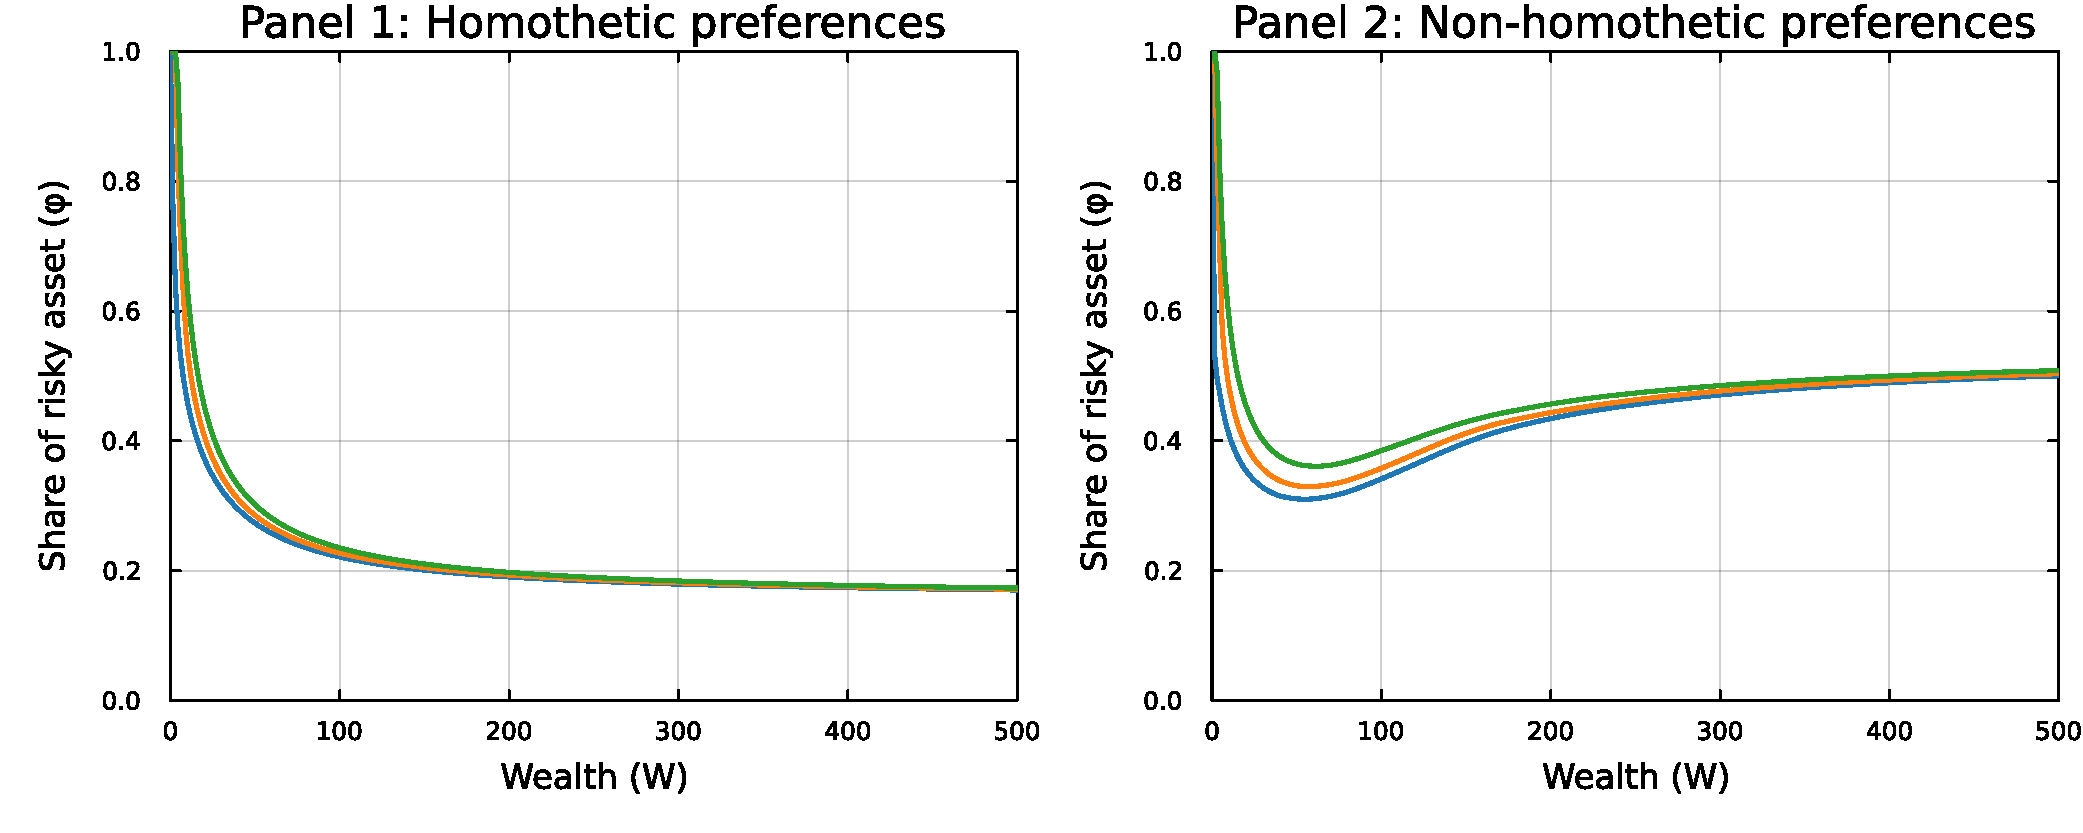
\includegraphics[width=1.0\textwidth]{figure_2.pdf}
    \caption{Portfolio shares for homothetic and non-homothetic preferences}
    \label{fig:risky_share}
\end{figure}

What is crucial for applying the formula to the dynamic setting is that the "wealth" of an agent consists not only of the financial assets they hold. Future discounted income, sometimes called the "human wealth", is also considered while choosing an investment portfolio. Since this is a relatively safe "asset", as the autocorrelation is high, standard deviation is limited, and under a discretized Markov process, it does not fall below the value of the lowest state, the agents with the lowest financial wealth tend to choose the highest share of risky financial assets. For homothetic preferences, as shown in Panel~1 of \autoref{fig:risky_share}, the risky share decreases and converges to the value of the M-S share for $\theta$. In contrast, for Straub preferences (Panel~2), after an initial drop, the risky share rises.

\subsection{Full model}

Now I move to the full partial equilibrium framework that I will use to generate the stationary distribution and analyze cross-sectional quantities for saving behavior and portfolio choice.

\textbf{Preferences.} Because of the well-known issue in macro-finance literature of the equity premium puzzle \parencite{mehra1985}, standard CRRA preferences are not able to generate realistic investment behavior for empirically observed risk-free rate, risk premium, and equity volatility. This also concerns Straub preferences. Therefore, I integrate the approaches of Straub and Epstein-Zin, where the latter is widely used to disentangle risk aversion and intertemporal elasticity of substitution. That allows for a realistic calibration of risk aversion while keeping the intertemporal choice unaffected. The preferences are given by recursive utility:
\begin{align*}
V\left(W_t^i, z_t^i\right) = \max_{\substack{\varphi_t^i \in [0,1] \\ c_t^i \in [0, \, W_t^i + w_tz_t^i]}} 
\Bigg\{ &
(1 - \gamma)(1 - \beta) \left(c_t^i\right)^{1 - \rho} + (1 - \gamma) \beta 
\left( \mathbb{E}_t \left[ V\left(W_{t+1}^i, z_{t+1}^i\right)^{1 - \theta} \right] \right)^{\frac{1 - \rho}{1 - \theta}} \\
& + \gamma (1 - \beta) \frac{1 - \rho}{1 - \eta} 
\, A \left(W_t^i + \overline{W} \right)^{1 - \eta}
\Bigg\}^{\frac{1}{1 - \rho}}
\end{align*}

Here $\theta$ is risk aversion, and $\rho$ is the inverse of the intertemporal elasticity of substitution. $\eta$ is the parameter for utility from bequests as before, and $\eta<\rho \leq \theta$. The parameters multiplying utility from bequests ensure that the Euler Equation nests the model from Section~\ref{subsec:simple_model} as a special case when $\rho = \theta$. $\overline{W}$ is the "subsistence" level of wealth, which shifts the marginal utility. It makes bequests even more "luxury", but also, more importantly, allows agents to hold zero wealth, which is important for matching wealth shares.

\textbf{Agent optimization problem.} Agents are not allowed to get into debt, which imposes the savings level to be non-negative. Short sale is also prohibited, so the risky asset share has to be between 0 and 1. Because of the human wealth effect of very high risky shares for the lowest values of wealth, I add the stock market participation cost $\kappa$ that the agent has to pay each period to invest in risky assets. It discourages the poorest agents from investing, as the gains they can obtain from the stock market are relatively small in absolute terms. The budget constraint is hence:

\[
w_t z_t^i + W_t^i = c_t^i + s_t^i + \mathbbm{1}_{\{\varphi_t^i > 0\}} \kappa
\]
And the full recursive agent problem is:
\begin{align*}
V\left(W_t^i, z_t^i\right) = \max_{\substack{\varphi_t^i \in [0,1] \\ c_t^i \in [0, \, W_t^i + w_tz_t^i]}} 
\Bigg\{ &
(1 - \gamma)(1 - \beta) \left(c_t^i\right)^{1 - \rho} + (1 - \gamma) \beta 
\left( \mathbb{E}_t \left[ V\left(W_{t+1}^i, z_{t+1}^i\right)^{1 - \theta} \right] \right)^{\frac{1 - \rho}{1 - \theta}} \\
& + \gamma (1 - \beta) \frac{1 - \rho}{1 - \eta} 
\, A \left(W_t^i + \overline{W} \right)^{1 - \eta}
\Bigg\}^{\frac{1}{1 - \rho}} \\
\text{s.t.} \quad 
& w_t z_t^i + W_t^i = c_t^i + s_t^i + \mathbbm{1}_{\{\varphi_t^i > 0\}} \kappa \\
& RET_{t+1}^i=(1-\varphi_t^i) R_{t+1} + \varphi_t^i(1+d_{t+1}^i) \\
& W_{t+1}^i = RET_{t+1}^i s_t^i \\
& s_t^i \geq 0 \\
& \varphi \in [0,1]
\end{align*}

The full derivation of the Euler Equation is contained in Appendix~\ref{app:euler}. The equation is:
\begin{align*}
\left(c_t^i\right)^{-\rho} 
&= \beta \, \mathbb{E}_t \Bigg[
    \left( 
        (1 - \gamma) \left(c_{t+1}^i\right)^{-\rho} 
        + \gamma A\left(W_{t+1}^i + \overline{W} \right)^{-\eta} 
    \right) \notag \\[1ex]
&\quad \cdot 
    \left(
        \frac{
            V\left(W_{t+1}^i, z_{t+1}^i\right)
        }{
            \left( \mathbb{E}_t \left[ V\left(W_{t+1}^i, z_{t+1}^i\right)^{1 - \theta} \right] \right)^{\frac{1}{1 - \theta}}
        }
    \right)^{\rho - \theta}
    RET_{t+1}^i
\Bigg]
\end{align*}

It clearly shows that, indeed, under $\rho = \theta$ the Epstein-Zin "wedge" disappears and the equation is exactly as in Section~\ref{subsec:simple_model}. The same concerns the portfolio choice:
\begin{align*}
\mathbb{E}_t \Bigg[
    \left( 
        (1 - \gamma) \left(c_t^i\right)^{-\rho} 
        + \gamma A\left(W_{t+1}^i + \overline{W} \right)^{-\eta} 
    \right)
    V\left(W_{t+1}^i, z_{t+1}^i\right)^{\rho - \theta}
    \left(1 + d^i - R \right)
\Bigg] = 0 \label{eq:ret_cond}
\end{align*}

It is, however, valid only if the expected value function stemming from a diversified portfolio exceeds the expected value function under $\varphi_t^i=0$ when the agent does not pay the participation cost.

\textbf{Stochastic processes.} Individual labor productivity is stochastic and comprises two components. The first corresponds to a set of "normal" productivity states that follow a discrete Markov process with log-normal distribution with standard deviation $\sigma_z$ and persistence parameter $\rho_z$. The second is a high-productivity state, calibrated in the spirit of \textcite{castaneda2003}, and represents the top 5\% of earners in the income distribution. Agents in this state receive labor income equal to $z_{top}$ times the average income of agents in the remaining 95\%. The probability of remaining in the high-productivity state is $\rho_{top}$, while the transition probability from any normal state to the high-productivity state is uniform and chosen such that 5\% of agents occupy the high-productivity state in the stationary distribution.

The return on the risky asset, denoted $d_t^i$, is also governed by a two-component process. With probability $p_B$, the firm in which the agent invests goes bankrupt, resulting in a total loss of the investment, i.e., $d_t^i = -1$. With the remaining probability $1 - p_B$, the return is drawn from a log-normal distribution with standard deviation $\sigma_d$ and a mean calibrated to ensure that the expected return across the entire process equals $E_d$.

\textbf{Macro environment.} Time is discrete and indexed by $t$, one period corresponds to one year. The economy is populated by a continuum of agents of measure 1. As introduced earlier, each period, an agent dies with probability $\gamma$. In standard fashion, the dynasty is immediately replaced by an offspring who inherits both the parent’s wealth and productivity state, preserving intergenerational continuity.

To prevent excessive wealth concentration and to guarantee the existence of a stationary distribution, I introduce a stochastic mechanism of dynastic renewal. With probability $\xi$, which I refer to as the fortune destruction probability, the lineage is terminated entirely and replaced by a newly born agent. This new agent enters the economy with wealth equal to the current average wealth in the population and with a productivity state drawn from the stationary distribution of the idiosyncratic income process. This "fortune destruction" can be interpreted as a certain individual dying without descendants, donating all their wealth to charity, or an irresponsible inheritor squandering the family fortune.

This mechanism captures a range of empirically observed real-world phenomena that interrupt the dynastic persistence of wealth. As documented by \textcite{benhabib2017}, extremely high persistence in wealth accumulation can lead to the formation of "wealth traps" or Pareto tails with infinite variance unless mechanisms of dispersion are introduced. Similarly, \textcite{gabaix2009} shows that to generate stationary distributions with realistic tail exponents, models often require stochastic reset mechanisms or entry-exit dynamics. The $\xi$-process used here parallels such approaches.

\section{Calibration}
\label{sec:calibration}

\subsection{Parameters Set from the Literature and Empirical Evidence}

The mortality rate $\gamma$ is set to 2\%, implying an expected productive lifespan of 50 years. The "fortune destruction" parameter is set to $\xi = 0.01$ to ensure the existence of a stationary wealth distribution and prevent divergence of wealth accumulation. This value is close to $\xi = 0.005$ used by \textcite{benhabib2017}.

The persistence and volatility of the income process are set to $\rho_z = 0.95$ and $\sigma_z = 0.1$, which are standard in the literature. The relative earnings of high-income individuals are set to $z_{\text{top}} = 6$, reflecting a sixfold income ratio between the top 5\% earners and the rest, consistent with the estimates reported by \textcite{piketty2018}. The persistence of the high-productivity state is calibrated such that its expected duration is approximately 20 years, in line with one of the values used by \textcite{benhabib2019}.

The return of safe assets is $R=1.015$, consistent with the typical range of 1–2\% found in the literature. In particular, this value aligns with the estimate of 1.6\% based on PSID data by \textcite{gourinchas2002}. The average return on the risky asset is set to $E_d = 0.065$, implying an equity premium of 5\%. This value balances empirical estimates of approximately 6\% with the lower 3–4\% figures typically used in structural models \parencite{mehra1985, bansal2004, barro2006}.

The standard deviation of risky returns is set to $\sigma_d = 0.2$, matching historical volatility of the S\&P 500 \parencite{ibbotson2018} and closely aligned with the 18.5\% used by \textcite{cochrane2005}. Finally, the probability of firm bankruptcy is set to $p_B = 0.01$, in line with empirical estimates for public companies in the U.S., and consistent with the probability of rare disasters in \textcite{barro2006}.

\subsection{Internally Calibrated Parameters}

The model is calibrated to replicate key features of the contemporary U.S. economy. Wages are normalized to $w = 1$. The preference parameters $\theta$, $\rho$, $\eta$, and $A$ are jointly calibrated to match the observed concentration of wealth among the richest households. The "subsistence" wealth level $\overline{W}$ is chosen to replicate the empirical share of wealth held by the bottom 50\% of the population.

The discount factor is set to $\beta = 0.955$, so that the model reproduces the empirical median wealth of approximately $2.3 \times w$. The fixed participation cost for risky asset markets, $\kappa = 0.2$, is calibrated to ensure that households in the bottom half of the wealth distribution opt out of equity investment.

\begin{table}[htbp]
\centering
\caption{Model Parameters: Values and Sources}
\label{tab:parameters}
\begin{adjustbox}{width=\textwidth}
\begin{tabular}{llll}
\toprule
\textbf{Symbol} & \textbf{Name} & \textbf{Value} & \textbf{Source / Target} \\
\midrule
\multicolumn{4}{l}{\textit{Externally Calibrated Parameters}} \\
\addlinespace
$\gamma$       & Mortality rate                   & 0.02    & Implies 50-year lifespan \\
$\xi$          & Fortune destruction rate         & 0.01    & Stationarity; \textcite{benhabib2017} \\
$\rho_z$       & Persistence of income            & 0.95    & Standard in literature \\
$\sigma_z$     & SD of income process             & 0.10    & Standard in literature \\
$z_{\text{top}}$ & Top income ratio               & 6       & \textcite{piketty2018} \\
$\rho_{\text{top}}$ & Persistence of top state    & 0.95    & \textcite{benhabib2019} \\
$R$            & Return on safe asset             & 1.015   & Standard; \textcite{gourinchas2002} \\
$E_d$          & Expected return on risky asset   & 0.065   & Equity premium $\approx 5\%$ \\
$\sigma_d$     & SD of risky returns              & 0.20    & S\&P 500 volatility; \textcite{cochrane2005} \\
$p_B$          & Bankruptcy probability           & 0.01    & Public firms; \textcite{barro2006} \\
\midrule
\multicolumn{4}{l}{\textit{Internally Calibrated Parameters}} \\
\addlinespace
$w$            & Wage                             & 1       & Normalization \\
$\beta$        & Discount factor                  & 0.955    & Matches median wealth ($2.3 \times w$) \\
$\theta$       & CRRA                             & 10      & Matches top wealth shares \\
$\rho$         & Inverse of EIS                   & 4       & Matches top wealth shares \\
$\eta$         & Bequest elasticity               & 1.6     & Matches top wealth shares \\
$A$            & Bequest weight                   & 3.5     & Matches top wealth shares \\
$\overline{W}$ & Subsistence wealth               & 10      & Matches bottom 50\% wealth share \\
$\kappa$       & Stock participation cost         & 0.2     & Bottom 50\% opt out of risky assets \\
\bottomrule
\end{tabular}
\end{adjustbox}
\end{table}


\section{Quantitative analysis}
\label{sec:analysis}

I solve the model numerically using the Endogenous Grid Method (EGM), following the approach of \textcite{carroll2006}. Since the idiosyncratic return $RET_t^i$ is stochastic and the standard EGM relies on deterministic returns to construct the endogenous grid, I adapt the method using a double-interpolation approach, described in Appendix~\ref{app:egm_stoch}. The optimal portfolio share is determined by solving the first-order condition via bisection method. To compute the Epstein–Zin wedge consistently, I iterate the value function at each EGM step until it converges under the current consumption policy. As the entire algorithm avoids global numerical optimization, it remains computationally efficient and supports the use of a finely discretized state space.

\subsection{Results and Comparison to Data}

\subsubsection{Wealth Distribution}

The main focus of the calibration was to accurately reflect the wealth distribution, particularly the top wealth shares. As a result, the model closely matches relevant data moments, as shown in Table~\ref{tab:wealth_comparison}. Additionally, the Gini coefficient is nearly perfectly aligned with the data.

\begin{table}[htbp]
\centering
\caption{Wealth share by group: WID.world data versus model}
\label{tab:wealth_comparison}
\begin{tabular}{@{} lcc @{}}
\toprule
\textbf{Wealth group} & \textbf{WID.world} & \textbf{Model} \\
\midrule
Bottom 50\%      & $<2\%$  & 2\%   \\
Top 50\%         & $>98\%$ & 98\%  \\
Top 10\%         & 78\%    & 73\%  \\
Top 1\%          & 38\%    & 33\%  \\
Top 0.1\%        & 18\%    & 18\%  \\
\hline
Gini coefficient & 0.83    & 0.80  \\
\bottomrule
\end{tabular}

\vspace{0.5em}
\begin{minipage}{0.9\linewidth}
\small Source: \textcite{wid2023}.
\end{minipage}
\end{table}


To capture the absolute quantities of wealth distributions, I use the average wage (normalized to 1 in the model) as a benchmark. According to data from the Bureau of Labor Statistics, the average wage per worker in 2023 was \$65,000 \parencite{bls_2023}. The median household net worth in 2022 was \$192,000, as reported by the Survey of Consumer Finances \parencite{scf2022}. Since the average household has 1.3 earners \parencite{uscensus2022}, I assume a ratio of 2.3 between median wealth and the wage ($w$) as a reasonable approximation of recent values.

In terms of average household wealth, the SCF 2022 reports a value of \$1.06 million, while the SCF 2019 reports \$747,000 (or approximately \$866,000 when adjusted for inflation). These figures imply a ratio of average wealth to average wage in the range of 10.2 to 12.5. This in principle agrees with the value implied by the model, which is 10.5.

\subsubsection{Portfolio choice}

As shown in Section~\ref{subsec:simple_model}, the share of risky assets increases with wealth under Straub preferences. This increase is particularly pronounced for the middle segment of the wealth distribution and tends to level off at higher wealth levels. The relatively high risky asset share among poorer agents is now partially mitigated by the introduction of a participation cost $\kappa$. However, calibrating $\kappa$ to match precisely the observed participation rate within the middle 40\% of the wealth distribution proves challenging: for higher values of $\kappa$, participation is nearly zero, while for lower values, it becomes implausibly high. For this reason, I focus on capturing the behavior of wealthier agents and allow most low- and middle-wealth agents to remain out of the risky asset market.

Table~\ref{tab:return} compares the model's outcomes with data from the Federal Reserve's Distributional Financial Accounts (DFA) for 2022. I classify "Corporate equities and mutual fund shares" as well as "Private businesses" as risky assets, measured relative to total assets. The model performs well in replicating the risky asset share held by the top 10\% of the wealth distribution, with the exception of the richest 1\%. Accurately reproducing the extremely high risk exposure of this group would, under the assumed risk premium, imply excessively high returns, preventing the existence of a stationary wealth distribution.

\begin{table}[htbp]
\centering
\caption{Risky share and average return by group: DFA data versus model}
\label{tab:return}
\begin{tabular}{@{} lcc @{}}
\toprule
\textbf{Wealth group} & \textbf{DFA} & \textbf{Model}  \\
\midrule
Bottom 50\%      & 5\%   & 0\% \\
Middle 40\%      & 13\%  & 1\% \\ 
90\% - 99\%      & 33\%  & 30\% \\
Top 1\%          & 60\%  & 30\% \\
\bottomrule
\end{tabular}

\vspace{0.5em}
\begin{minipage}{0.9\linewidth}
\small Source: \textcite{dfa2024}.
\end{minipage}
\end{table}

\subsection{Model Dynamics}

\subsubsection{Feedback Loop Mechanism}

Unlike many models that aim to replicate the empirical wealth distribution, the present framework does not rely on ex-ante heterogeneity - such as differences in discount factors, permanent productivity levels, or privileged access to high-return investments - nor does it assume large and persistent stochastic income shocks ("divine states"). Instead, it seeks to demonstrate that substantial and persistent wealth inequality can emerge even among agents who are nearly identical in their fundamentals. The only deviation from full symmetry is the inclusion of a mildly asymmetric income process, featuring a high-income state assigned to a small fraction of agents (top 5\%).

The core mechanism operates through the interaction of non-homothetic preferences and endogenous portfolio choice. The Straub-type utility specification generates declining marginal propensities to consume (MPCs), implying that wealthier agents systematically save a larger fraction of their income. This endogenous saving gradient leads to self-reinforcing accumulation: agents who are marginally wealthier in one period tend to grow wealthier in the next. However, while this channel alone does generate upward drift in wealth among the rich, its force is inherently constrained by the relatively small share of consumption at the top of the distribution, even under homothetic preferences.

The dynamic changes significantly when portfolio choice is introduced. Due to lower relative risk aversion, wealthier agents allocate a larger fraction of their assets to risky investments with higher expected returns. This leads to a scale-dependent rate of return on wealth: the rich not only save more, but also earn more on their savings. This dual advantage accelerates wealth accumulation at the top and generates long-run disparities that are consistent with empirical data. Crucially, in the absence of redistributive forces or mechanisms of “fortune destruction,” this feedback loop - where higher wealth enables both greater saving and access to superior returns - can give rise to extreme and self-perpetuating inequality. Over time, even minor initial differences can compound into vast and structurally entrenched disparities, illustrating how a system governed by seemingly neutral rules may still harbor powerful dynamics of cumulative advantage - perhaps the most fundamental "spirit of capitalism".

\subsubsection{Social Mobility}

To assess social mobility within the model, I conduct the following experiment. Given the policy functions for consumption ($c$) and risky asset holdings ($\phi$), I simulate stochastic paths of labor income shocks and realized returns on risky assets. This procedure is repeated 100,000 times to generate a robust distribution of outcomes. The results are presented in \autoref{fig:mobility}, which displays the probability that, after a given number of periods, an agent who starts with wealth corresponding to a specific percentile will be found in a particular wealth group.

\begin{figure}[h]
    \centering
    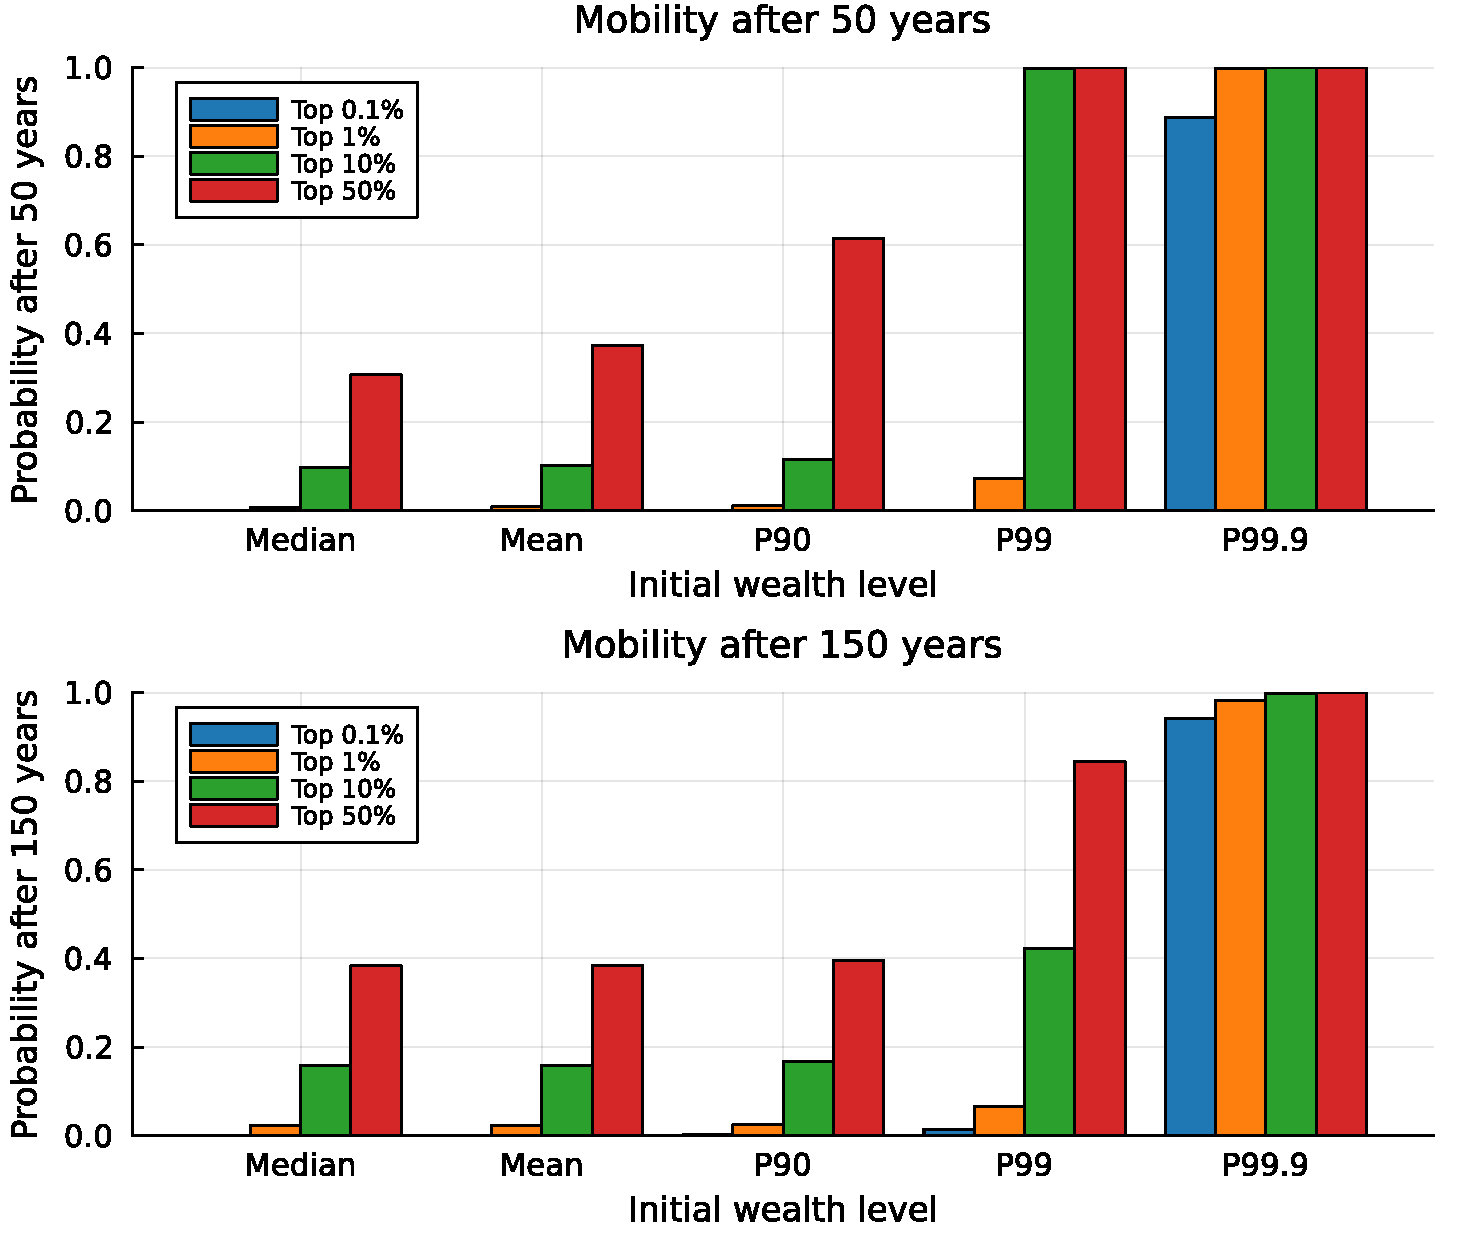
\includegraphics[width=1.0 \textwidth]{figure_3.pdf}
    \caption{Probability of transitioning into selected wealth percentiles after 50 and 150 periods, conditional on initial wealth rank.}
    \label{fig:mobility}
\end{figure}

The figure includes two panels, corresponding to horizons of 50 and 150 years—approximately one and three generations, respectively. This allows for the analysis of both short-run intergenerational mobility (i.e., the chances for upward mobility of a newly “born” agent) and long-run persistence of wealth, reflecting the extent to which economic status remains influenced by more distant ancestors.

The most striking feature of the simulated mobility patterns is the extreme persistence of wealth among the top 0.1\%. An agent starting in this group almost never exits it, even over a long horizon. High returns on their wealth allow them to remain in the economic elite despite adverse income or asset return shocks. For the rest of the population, however, the prospect of joining this top fraction is virtually nonexistent. Within a single generation, the probability of entering the top 0.1\% is effectively zero for agents outside it; even over three generations, this probability remains around 0.1 - 0.3\% for those in the bottom 99\% of the wealth distribution, and only around 1.5\% for agents starting from the 99th percentile.

\begin{table}[htbp]
\centering
\caption{Quantiles of the wealth distribution}
\label{tab:quantlies}
\begin{tabular}{@{} lcc @{}}
\toprule
\textbf{Statistic} & \textbf{Wealth Level} & \textbf{Ratio to Median} \\
\midrule
Median      &  2.3  & 1.00  \\
Mean        &  10.5 & 4.53  \\
P90         &  19.7 & 8.47  \\
P99         &  111  & 47.6  \\
P99.9       &  406  & 174.8 \\
\bottomrule
\end{tabular}
\vspace{0.5em}
\end{table}


This result reflects a deeper structural distinction within the upper tail of the distribution. Most of the top 1\%, while still relatively affluent, are significantly closer - both in economic position and in upward potential - to the upper middle class than to the very top. This is further illustrated by their much lower persistence: an individual born into the 99th percentile has only about a 8\% chance of remaining in the top 1\% by the end of life. This underscores the distinction between the ultra-wealthy and the rest of the upper class.

At the lower end of the distribution, the model does not fully capture the observed dynamics of social mobility. This is primarily due to the simplified treatment of the income process, particularly its persistence, which plays a crucial role in shaping mobility for lower- and middle-wealth agents. As a result, the upward prospects of individuals in the 90th percentile are not meaningfully different from those around the median or mean. A richer income process that incorporates features such as a fixed productivity component or greater skewness, such as the one proposed by \textcite{benhabib2019}, would likely offer a more accurate account of transitional dynamics in these segments of the population.

\subsection{Alternative Specifications}

To assess the joint importance of non-homothetic preferences and endogenous portfolio choice in shaping the wealth distribution, I perform a model-based decomposition exercise. Specifically, I compare the baseline specification with two alternative variants in which these mechanisms are selectively deactivated. The first alternative includes portfolio choice but omits utility from bequests, thereby eliminating the saving motive that generates declining marginal propensities to consume across the wealth distribution. The second maintains non-homothetic preferences but restricts households to a single asset corresponding to a fixed and identical portfolio across agents (risky asset share is set to the average level for baseline model).

\begin{table}[htbp]
\centering
\caption{Calibration of key parameters across models}
\label{tab:calibration_comparison}
\begin{tabular}{@{} lccc @{}}
\toprule
\textbf{Parameter} & \textbf{Baseline Model} & \textbf{Homothetic} & \textbf{Fixed Portfolio} \\
\midrule
$\beta$         & 0.955 & 0.961 & 0.955 \\
$\theta$        & 10    & 3     & 4     \\
$\rho$          & 4     & 3     & 4     \\
$\eta$          & 1.6   &  --   & 1.6   \\
$A$             & 3.5   &  --   & 4     \\
$\overline{W}$  & 10    &  --   & 10    \\
$\kappa$        & 0.2   & 0.3   &  --   \\
\bottomrule
\end{tabular}
\vspace{0.5em}
\end{table}

The models are calibrated primarily to match the level of median assets, which serves as a common reference point for comparison. This target primarily determines the discount factor, though it also influences the intertemporal elasticity of substitution (particularly in the homothetic specification). Parameters of the utility function are chosen to replicate the observed wealth distribution as closely as each specification permits, with special attention to matching the concentration of wealth in the top percentiles.

\begin{table}[htbp]
\centering
\caption{Comparison of results across models}
\label{tab:results_comparison}
\begin{tabular}{@{} lcccc @{}}
\toprule
\textbf{Moment} & \textbf{Data} & \textbf{Baseline Model} & \textbf{Homothetic} & \textbf{Fixed Portfolio} \\
\midrule
Median assets to $w$     & 2.3  & 2.3   & 2.0   & 2.3   \\
Mean assets to $w$       & 12.5 & 10.5  & 15.2  & 6.9   \\
Gini coefficient         & 0.83 & 0.80  & 0.82  & 0.73  \\
Bottom 50\% wealth share & 2\%  & 2\%   & 1\%   & 4\%   \\
Top 50\% wealth share    & 98\% & 98\%  & 99\%  & 96\%  \\
Top 10\% wealth share    & 78\% & 73\%  & 73\%  & 65\%  \\
Top 1\% wealth share     & 38\% & 33\%  & 26\%  & 16\%  \\
Top 0.1\% wealth share   & 18\% & 18\%  & 7\%   & 2.4\% \\
\bottomrule
\end{tabular}
\vspace{0.5em}
\end{table}

The implications for inequality are significant. The baseline model closely replicates the empirical distribution, producing a Gini coefficient of 0.80, a top 1\% wealth share of 33\%, and a top 0.1\% share of 18\%, all closely aligned with survey data. In contrast, the homothetic model, despite producing a slightly higher mean wealth, overconcentrates wealth at the very top (top 1\% share drops to 26\%, and top 0.1\% to 7\%), failing to match the long tail of the distribution. Meanwhile, the fixed-portfolio specification understates inequality across the board, with a top 1\% share of only 16\% and top 0.1\% of just 2.4\%, indicating that portfolio composition plays an important role in amplifying disparities.

It is worth noting that in the homothetic model, wealth inequality is driven primarily by the participation cost. When $\kappa$ is set to zero,\footnote{Due to the low skewness of the resulting distribution, it is not possible to simultaneously match the empirical median asset level of 2.3 and obtain a reasonable mean: see Appendix.} the Gini coefficient drops to 0.58, and the wealth shares of the top 1\% and top 0.1\% are reduced by approximately two-thirds (full calibration details and results are provided in Appendix~\ref{app:alt_cali}). In contrast, removing the participation cost in the baseline model ($\kappa = 0$) yields less dramatic changes, with the top 1\% and 0.1\% wealth shares falling to 24\% and 14\%, respectively.

The fixed portfolio model (with Straub preferences but no portfolio choice) produces an even less skewed distribution than the homothetic specification - at least in terms of the upper tail - though it exhibits larger disparities between the lower and middle segments of the distribution. Interestingly, assigning a very low value to the bequest utility parameter $\eta$ can restore a heavy-tailed distribution, with the top 1\% and 0.1\% holding 34\% and 16\% of wealth, respectively. This suggests that the role of risk aversion in shaping inequality is dependent on parametrization. However, such a low $\eta$ also implies an implausibly flat consumption profile: in this calibration, the richest 0.1\% consume only about six times more than the poorest agents, making the baseline model more realistic overall.

\section{Conclusion}
\label{sec:conclusion}

This paper  sheds new light on the mechanisms underlying the distribution of wealth, especially regarding the disproportionate share held by the richest households. Rather than attributing top wealth concentration to exogenous heterogeneity in preferences or productivity, the model emphasizes an endogenous, self-reinforcing mechanism: wealthier agents not only save a larger share of their income, but - due to lower relative risk aversion - also obtain higher average returns on their assets through greater exposure to risky investments. This dual dynamic generates a powerful feedback loop that amplifies and entrenches inequality over time.

By embedding Straub-type non-homothetic preferences and Epstein-Zin recursive utility into a standard Aiyagari framework with portfolio choice, the model replicates key features of the empirical U.S. wealth distribution. In particular, it matches the pronounced concentration of wealth among the top percentiles, the increasing share of risky assets with wealth, and the resulting wealth-return gradient observed in microdata.

Simulations reveal not only the distributional implications of these mechanisms but also their dynamic consequences for social mobility. The model uncovers extreme persistence at the top: agents starting in the top 0.1\% remain there with near certainty, while upward mobility into this elite group is virtually nonexistent, even over multiple generations.

Counterfactual simulations underscore the critical importance of both declining marginal propensities to consume and endogenous portfolio choice in generating realistic levels of inequality. When either of these mechanisms is removed, the model's ability to match the observed concentration of wealth—particularly at the very top—deteriorates significantly. These findings highlight the necessity of incorporating dynamic investment behavior and heterogeneity in saving motives to fully capture the mechanisms through which wealth accumulates and concentrates across the distribution.

Looking ahead, a natural extension of the present analysis involves embedding the model within a general equilibrium framework. This would enable the evaluation of policy interventions - particularly redistributive measures such as wealth or capital gains taxation - within a fully endogenous setting. One especially promising direction is to interpret the risky asset as equity shares in firms generating monopolistic profits. Such a formulation would directly connect the literature on wealth inequality with that on market power, a connection that has become increasingly relevant as the profit share in GDP exceeds 20\% in many advanced economies. Given the observable link between the largest fortunes and firms with significant market dominance, a deeper analysis of how rising markups since the 1980s have contributed to wealth concentration appears both timely and necessary.

Finally, I wish to emphasize a methodological issue that is inherently tied to models featuring feedback between wealth and its return. The framework of stationary distributions, widely adopted since the earliest heterogeneous-agent models due to its computational tractability, appears increasingly inadequate for contemporary analysis. The assumption that today’s wealth distribution is either near its steady state or merely perturbed by exogenous shocks is becoming more difficult to defend. As shown in the influential analysis by \textcite{hubmer2021}, the U.S. economy appears to be on a prolonged transition path, far from stationarity - even if one assumes it had started from such a state by the 1960s. It may well be that advances in machine learning techniques for solving dynamic optimization problems with infinite state spaces \parencite{maliar2021, fernandez2024}, or a departure from the rational expectations paradigm - which increasingly constitutes a constraint rather than a convenience (as argued by \textcite{moll2024}) - could provide a path forward. These approaches may enable us to abandon the axiomatically imposed assumption of stationarity and arrive at qualitatively new insights into the dynamics of inequality.

\printbibliography[title={Bibliography}]

\appendix
\section*{Appendix}
\addcontentsline{toc}{section}{Appendix}
\section{Derivation of the Euler Equation}
\label{app:euler}

Differentiation recursive value function with respect to $c_t^i$ and $\varphi_t^i$ gives the First Order Conditions:
\begin{align}
(1 - \beta) \left(c_t^i\right)^{-\rho} 
&= \beta 
\left( 
    \mathbb{E}_t \left[ V\left(W_{t+1}^i, z_{t+1}^i\right)^{1 - \theta} \right] 
\right)^{\frac{1 - \rho}{1 - \theta} - 1} \cdot \notag \\[1ex]
&\quad 
\mathbb{E}_t \left[ 
    V\left(W_{t+1}^i, z_{t+1}^i\right)^{-\theta} 
    V_W\left(W_{t+1}^i, z_{t+1}^i\right) 
    RET_{t+1}^i 
\right] \label{eq:euler_main} \\[1ex]
0 &= 
\mathbb{E}_t \left[ 
    V_W\left(W_{t+1}^i, z_{t+1}^i\right) 
    V\left(W_{t+1}^i, z_{t+1}^i\right)^{-\theta} 
    \left( 1 + d^i - R \right) 
\right] \label{eq:euler_risky}
\end{align}

Where $V_W$ denotes the derivative of the value function over the first argument. From the Envelope Theorem:
\begin{align}
V_W\left(W_t^i, z_t^i\right) = 
&\left[
    (1 - \gamma)(1 - \beta) \left(c_t^i\right)^{1 - \rho} 
    + \beta 
    \left( \mathbb{E}_t \left[ V\left(W_{t+1}^i, z_{t+1}^i\right)^{1 - \theta} \right] \right)^{\frac{1 - \rho}{1 - \theta}} \right. \notag \\[1ex]
&\left. 
    + \gamma (1 - \beta) A\left(W_t^i + \overline{W}\right)^{\eta (1 - \rho)} 
\right]^{\frac{\rho}{1 - \rho}} \Bigg(
    (1 - \gamma) \beta 
    \left( \mathbb{E}_t \left[ V\left(W_{t+1}^i, z_{t+1}^i\right)^{1 - \theta} \right] \right)^{\frac{1 - \rho}{1 - \theta} - 1} \cdot \notag \\[1ex]
&    \mathbb{E}_t \left[ 
        V\left(W_{t+1}^i, z_{t+1}^i\right)^{-\theta} 
        V_W\left(W_{t+1}^i, z_{t+1}^i\right) 
        RET_{t+1}^i 
    \right] \notag \\[1ex]
&\quad + \gamma (1 - \beta) A\left(W_t^i + \overline{W} \right)^{-\eta}
\Bigg) \label{eq:envelope}
\end{align}

Substituting the value function and equation~\eqref{eq:euler_main} into \eqref{eq:envelope} gives the following:
\begin{align}
V_W\left(W_t^i, z_t^i\right) = 
&\left[ V\left(W_t^i, z_t^i\right) \right]^{\rho} \Bigg(
    (1 - \gamma) (1 - \beta) \left(c_t^i\right)^{-\rho} 
 + \gamma (1 - \beta) A\left(W_t^i + \overline{W} \right)^{-\eta}
\Bigg) \label{eq:value_derivative}
\end{align}

This can be shifted by one time index and substituted back to \eqref{eq:euler_main} as follows:
\begin{align}
(1 - \beta) \left(c_t^i\right)^{-\rho} 
&= \beta 
\left( 
    \mathbb{E}_t \left[ V\left(W_{t+1}^i, z_{t+1}^i\right)^{1 - \theta} \right] 
\right)^{\frac{1 - \rho}{1 - \theta} - 1} \notag \\[1ex]
&\quad \mathbb{E}_t \Bigg[ 
     RET_{t+1}^i V\left(W_{t+1}^i, z_{t+1}^i\right)^{-\theta} 
    \left[ V\left(W_{t+1}^i, z_{t+1}^i\right) \right]^{\rho} 
   \cdot \notag \\[1ex]
&\qquad \left( 
        (1 - \gamma)(1 - \beta) \left(c_{t+1}^i\right)^{-\rho} 
        + \gamma (1 - \beta) A\left(W_{t+1}^i + \overline{W} \right)^{-\eta}
    \right)
\Bigg]
\end{align}

This finally gives the Euler Equation:

\begin{align}
\left(c_t^i\right)^{-\rho} 
&= \beta \, \mathbb{E}_t \Bigg[
    \left( 
        (1 - \gamma) \left(c_{t+1}^i\right)^{-\rho} 
        + \gamma A\left(W_{t+1}^i + \overline{W} \right)^{-\eta} 
    \right) \notag \\[1ex]
&\quad \cdot 
    \left(
        \frac{
            V\left(W_{t+1}^i, z_{t+1}^i\right)
        }{
            \left( \mathbb{E}_t \left[ V\left(W_{t+1}^i, z_{t+1}^i\right)^{1 - \theta} \right] \right)^{\frac{1}{1 - \theta}}
        }
    \right)^{\rho - \theta}
    RET_{t+1}^i
\Bigg]
\end{align}

And from \eqref{eq:euler_risky} and \eqref{eq:value_derivative} I get the portfolio choice:
\begin{align}
\mathbb{E}_t \Bigg[
    \left( 
        (1 - \gamma) \left(c_t^i\right)^{-\rho} 
        + \gamma A\left(W_{t+1}^i + \overline{W} \right)^{-\eta} 
    \right)
    V\left(W_{t+1}^i, z_{t+1}^i\right)^{\rho - \theta}
    \left(1 + d^i - R \right)
\Bigg] = 0 \label{eq:ret_cond}
\end{align}

\section{Endogenous Grid Method with Stochastic Return}
\label{app:egm_stoch}

The usual framing of the EGM is that, having the future endogenous state variable (usually assets) value $a'$, we obtain the current consumption $c = g_c(a',z)$ from the Euler equation:

\begin{align}
    u_c(c) &= \beta R \mathbb{E}[u_c(c'(a',z'))] \\
    g_c(a',z)& = u_c^{-1} \left( \beta R \mathbb{E}[u_c(c'(a',z'))] \right) \label{eq:policy_basic}
\end{align}

and the current assets from the budget constraint:

\begin{equation}
    a = \frac{a' + g_c(a',z) - z}{R}
\end{equation}

where $z$ is the current value of the exogenous state variable (productivity). This convention doesn't seem convenient for introducing any stochasticity in $R$: the current assets would be ambiguous, not allowing us to settle the updated policy function on any grid.

See, however, that we can frame it differently: let's switch the endogenous state variable to the gross savings (increased by the return) $A = Ra$. Then the budget constraint changes to: 

\begin{equation}
    A = \frac{A'}{R} + g_c(A',z) - z
\end{equation}

Notice now that it is equivalent to $A = a' + g_c(A',z) - z$. Also, let the policy function on consumption $c(A,z)$ take $A$ as an argument. Analogously to \eqref{eq:policy_basic}, we have then:

\begin{equation}
    g_c(A',z) = u_c^{-1} \left( \beta R \mathbb{E}[u_c(c'(A',z'))] \right)
\end{equation}

To highight that $A'$ implicitly requires the knowledge of $R$, we can define:

\begin{equation}
    \hat{g}_c(a',z) = g_c(A',z) = u_c^{-1} \left( \beta R \mathbb{E}[u_c(c'(A',z'))] \right) = u_c^{-1} \left( \beta R \mathbb{E}[u_c(c'(R a',z'))] \right)
\end{equation}

which results in the budget constraint being
\begin{equation}
    A = a' + \hat{g}_c(a',z) - z \label{eq:constraint}
\end{equation}

We may then use the standard way of discretizing this function on a finite grid for $a$ and $z$:

\begin{equation}
    \hat{g}_c(a_i, z_j) = u_c^{-1} \left( \beta R \sum_{l=1}^{n_z} \Gamma_{j,l} u_c \left( c'(R a_i, z_l) \right) \right)
\end{equation}

where we obtain $c'(R a_i, y_l)$ by interpolating on the current policy function. This additional interpolation is obviously redundant for the deterministic $R$ case, but I will now show that it allows for $R$ to be random.

We are now ready to set the problem with stochastic $R$. The Euler equation is:

\begin{equation}
    u_c(c) = \beta \mathbb{E}[R' u_c(c'(A',z'))]
\end{equation}

 letting us find the updated policy function:

\begin{equation}
    \hat{g}_c(a',z) = u_c^{-1} \left( \beta \mathbb{E}[R' u_c(c'(R' a',z'))] \right)
\end{equation}

In the discretized version:

\begin{equation}
    \hat{g}_c(a_i, z_j) = u_c^{-1} \left( \beta \sum_{k=1}^{n_R}  \sum_{l=1}^{n_z} p_{R_k} R_k \Gamma_{j,l} u_c \left( c'(R_k a_i, z_l) \right) \right)
\end{equation}

where $p_{R_k}$ is the probability of a certain value of the interest rate. After getting this policy function, we interpolate it back on the grid $A_i$ constructed from \eqref{eq:constraint}. This is our policy function for an agent holding wealth $A_i$ at the beginning of the period, facing productivity shock $z_j$, and expecting future $R$ to be distributed according to  $p_{R_k}$.

\newpage

\section{Alternative Calibrations}
\label{app:alt_cali}

\begin{table}[htbp]
\centering
\caption{Comparison of calibration and results across six model variants}
\label{tab:model_scenarios}
\resizebox{\textwidth}{!}{%
\begin{tabular}{@{} l ccc ccc @{}}
\toprule
\textbf{Moment / Parameter} 
& \multicolumn{2}{c}{\textbf{Baseline}} 
& \multicolumn{2}{c}{\textbf{Homothetic}} 
& \multicolumn{2}{c}{\textbf{Fixed Portfolio}} \\
\cmidrule(lr){2-3} \cmidrule(lr){4-5} \cmidrule(lr){6-7}
& \textit{$\kappa=0.2$} & \textit{$\kappa=0$} 
& \textit{$\kappa=0.3$} & \textit{$\kappa=0$} 
& \textit{$\rho=1.6$} & \textit{$\rho=1.1$} \\
\midrule
$\beta$                     & 0.955 & 0.94 & 0.961 & 0.94 & 0.955 & 0.94 \\
$\theta$                    & 10    & 10    & 3     & 10     & 4     & 4     \\
$\rho$                      & 4     & 4     & 3     & 4     & 4     & 4     \\
$\eta$                      & 1.6   & 1.6   & --    & --    & 1.6   & 1.1   \\
$A$                         & 3.5   & 3.5   & --    & --    & 4.0   & 4.0   \\
$\overline{W}$              & 10    & 10    & --    & --    & 10    & 10    \\
$\kappa$                    & 0.2   & 0.0   & 0.3   & 0.0   & --    & --    \\
\midrule
\multicolumn{7}{c}{\textbf{Model outcomes}} \\
\midrule
Median assets to $w$        & 2.3   & 9.3   & 2.0   & 6.4   & 2.3   & 2.3   \\
Mean assets to $w$          & 10.5  & 16.9  & 15.2  & 10.8  & 6.9   & 11.9   \\
Gini coefficient            & 0.80  & 0.61  & 0.82  & 0.53  & 0.73  & 0.81  \\
Bottom 50\% wealth share    & 2\%   & 12\%  & 1\%   & 13\%  & 4\%   & 2\%   \\
Top 50\% wealth share       & 98\%  & 88\%  & 99\%  & 87\%  & 96\%  & 98\%  \\
Top 10\% wealth share       & 73\%  & 54\%  & 73\%  & 47\%  & 65\%  & 74\%  \\
Top 1\% wealth share        & 33\%  & 24\%  & 26\%  & 10\%  & 16\%  & 34\%  \\
Top 0.1\% wealth share      & 18\%  & 14\%  & 7\%   & 1.4\%   & 2.4\% & 16\% \\
\bottomrule
\end{tabular}%
}
\vspace{0.5em}
\begin{minipage}{0.95\linewidth}
\small\textit{Note:} Baseline models feature Straub preferences and endogenous portfolio choice. Homothetic models remove non-homotheticity. Fixed portfolio models eliminate portfolio choice while preserving bequest motives.
\end{minipage}
\end{table}



\end{document}
